\documentclass[11pt,a4paper]{article}
\usepackage[margin=0.85in]{geometry}
\usepackage[utf8]{inputenc}
\usepackage[T1]{fontenc}
\usepackage{hyperref}
\usepackage{graphicx}
\usepackage{tikz}
\usetikzlibrary{shapes,arrows,positioning,shadows,fit}
\usepackage{enumitem}
\usepackage{array}
\usepackage{longtable}
\usepackage{booktabs}
\usepackage{setspace}
\usepackage{makecell}
\usepackage{tabularx}
\usepackage{listings}
\usepackage{xcolor}
\usepackage{tcolorbox}

\definecolor{bg}{rgb}{0.95,0.95,0.92}

\hypersetup{
    colorlinks=true,
    linkcolor=blue,
    filecolor=blue,
    urlcolor=blue,
    citecolor=blue,
}

\usetikzlibrary{shapes,arrows,positioning,shadows,fit}
\onehalfspacing



\lstset{language=SQL,
    backgroundcolor=\color{bg}, 
    breaklines=true,
    frame=single,
    showspaces=false,
    showstringspaces=false,
    basicstyle=\ttfamily,
    numbers=left,
    numberstyle=\tiny,
    rulecolor=\color{black},
    keywordstyle=\color{blue},
    morekeywords={BEGIN, TRANSACTION, SAVEPOINT, ROLLBACK, TO, COMMIT, MODIFY, RENAME, COMMENT},
    commentstyle=\color{gray},
    captionpos=b
}


\begin{document}
\input{titlepage}
\newpage
\tableofcontents
\listoffigures
\listoftables
\newpage
\newpage

\section{System Architecture}

\subsection{Overview}

The healthcare web application follows a three-tier architecture pattern that separates the presentation layer, application logic layer, and data storage layer. This design provides clear separation of concerns, enhances maintainability, and supports independent development of frontend and backend components. The architecture enables parallel development, simplifies testing, and allows each tier to be updated independently.

\subsection{High-Level Architecture}

Figure~\ref{fig:architecture} illustrates the three-tier architecture of our system.

% [INSERT YOUR ARCHITECTURE DIAGRAM HERE]
\begin{figure}[htbp]
\centering
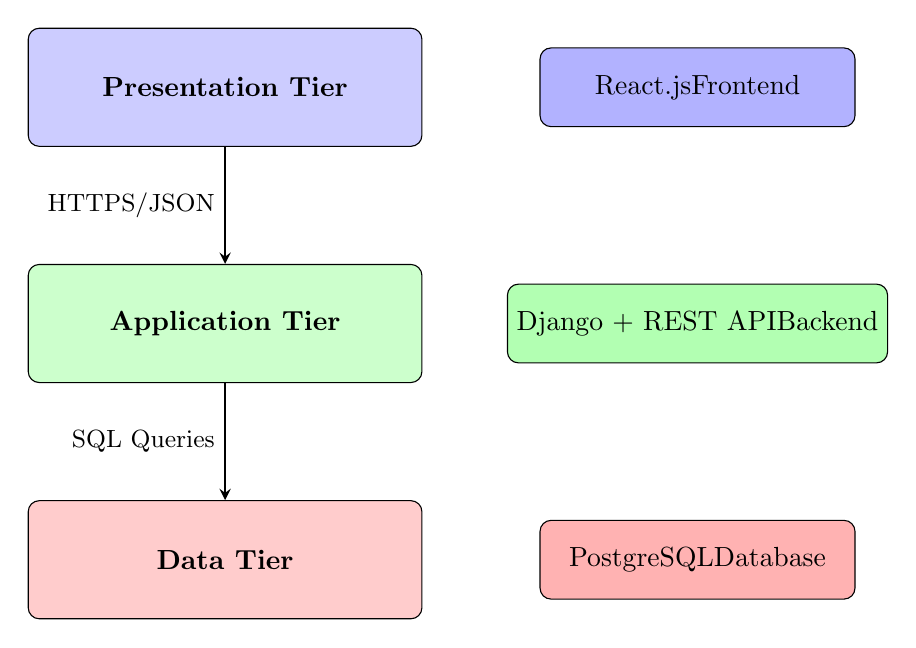
\begin{tikzpicture}[node distance=3cm, auto]
    % Define styles
    \tikzstyle{layer} = [rectangle, rounded corners, minimum width=5cm, minimum height=1.5cm, text centered, draw=black, fill=gray!10, font=\bfseries]
    \tikzstyle{component} = [rectangle, rounded corners, minimum width=4cm, minimum height=1cm, text centered, draw=black]
    \tikzstyle{arrow} = [thick,->,>=stealth]
    
    % Left side - Tiers
    \node [layer, fill=blue!20] (presentation) {Presentation Tier};
    \node [layer, fill=green!20, below of=presentation] (application) {Application Tier};
    \node [layer, fill=red!20, below of=application] (data) {Data Tier};
    
    % Right side - Technologies
    \node [component, fill=blue!30, right of=presentation, xshift=3cm] (react) {React.js\\ Frontend};
    \node [component, fill=green!30, right of=application, xshift=3cm] (django) {Django + REST API\\ Backend};
    \node [component, fill=red!30, right of=data, xshift=3cm] (postgres) {PostgreSQL\\ Database};
    
    % Vertical arrows between tiers
    \draw [arrow] (presentation) -- node[left, font=\small] {HTTPS/JSON} (application);
    \draw [arrow] (application) -- node[left, font=\small] {SQL Queries} (data);
    
\end{tikzpicture}
\caption{Three-Tier System Architecture}
\label{fig:architecture}
\end{figure}


\subsection{Architecture Components}

\subsubsection{Presentation Tier (Frontend)}

The presentation tier is built using React.js and runs in the user's web browser. It provides three separate interfaces for different user types: patients, doctors, and administrators.

\noindent
\textbf{Key Responsibilities:}
\begin{itemize}
    \item Display user interface components
    \item Handle user interactions and form inputs
    \item Validate user input before sending to backend
    \item Make asynchronous API calls to backend
    \item Update interface dynamically based on server responses
\end{itemize}

\noindent
\textbf{Technology:} React.js for component-based UI development and responsive single-page applications.

\subsubsection{Application Tier (Backend)}

The application tier is implemented using Django and Django REST Framework. It handles all business logic, authentication, and data processing.

\noindent
\textbf{Key Components:}
\begin{itemize}
    \item \textbf{URL Router:} Routes incoming requests to appropriate handlers
    \item \textbf{Authentication System:} Validates user tokens and manages sessions
    \item \textbf{Views:} Implement business logic and handle request processing
    \item \textbf{Serializers:} Convert data between JSON and Python objects
    \item \textbf{Models:} Define database structure using Django ORM
    \item \textbf{Permissions:} Enforce role-based access control
\end{itemize}

\noindent
\textbf{Technology:} Django and Django REST Framework for secure backend with built-in authentication, ORM, and robust API capabilities.

\subsubsection{Data Tier (Database)}

The data tier uses PostgreSQL to store all application data persistently.

\noindent
\textbf{Key Responsibilities:}
\begin{itemize}
    \item Store user accounts, patient profiles, medical records
    \item Execute SQL queries and return results
    \item Maintain data integrity through constraints
    \item Handle transactions and concurrent access
\end{itemize}

\noindent
\textbf{Technology:} PostgreSQL for reliable data storage with advanced features like JSON fields and array types useful for medical data.

\subsection{Request Flow Example}

Figure~\ref{fig:request-flow} illustrates the complete request flow when a patient books an appointment.

% [INSERT YOUR REQUEST FLOW DIAGRAM HERE]
\begin{figure}[htbp]
\centering
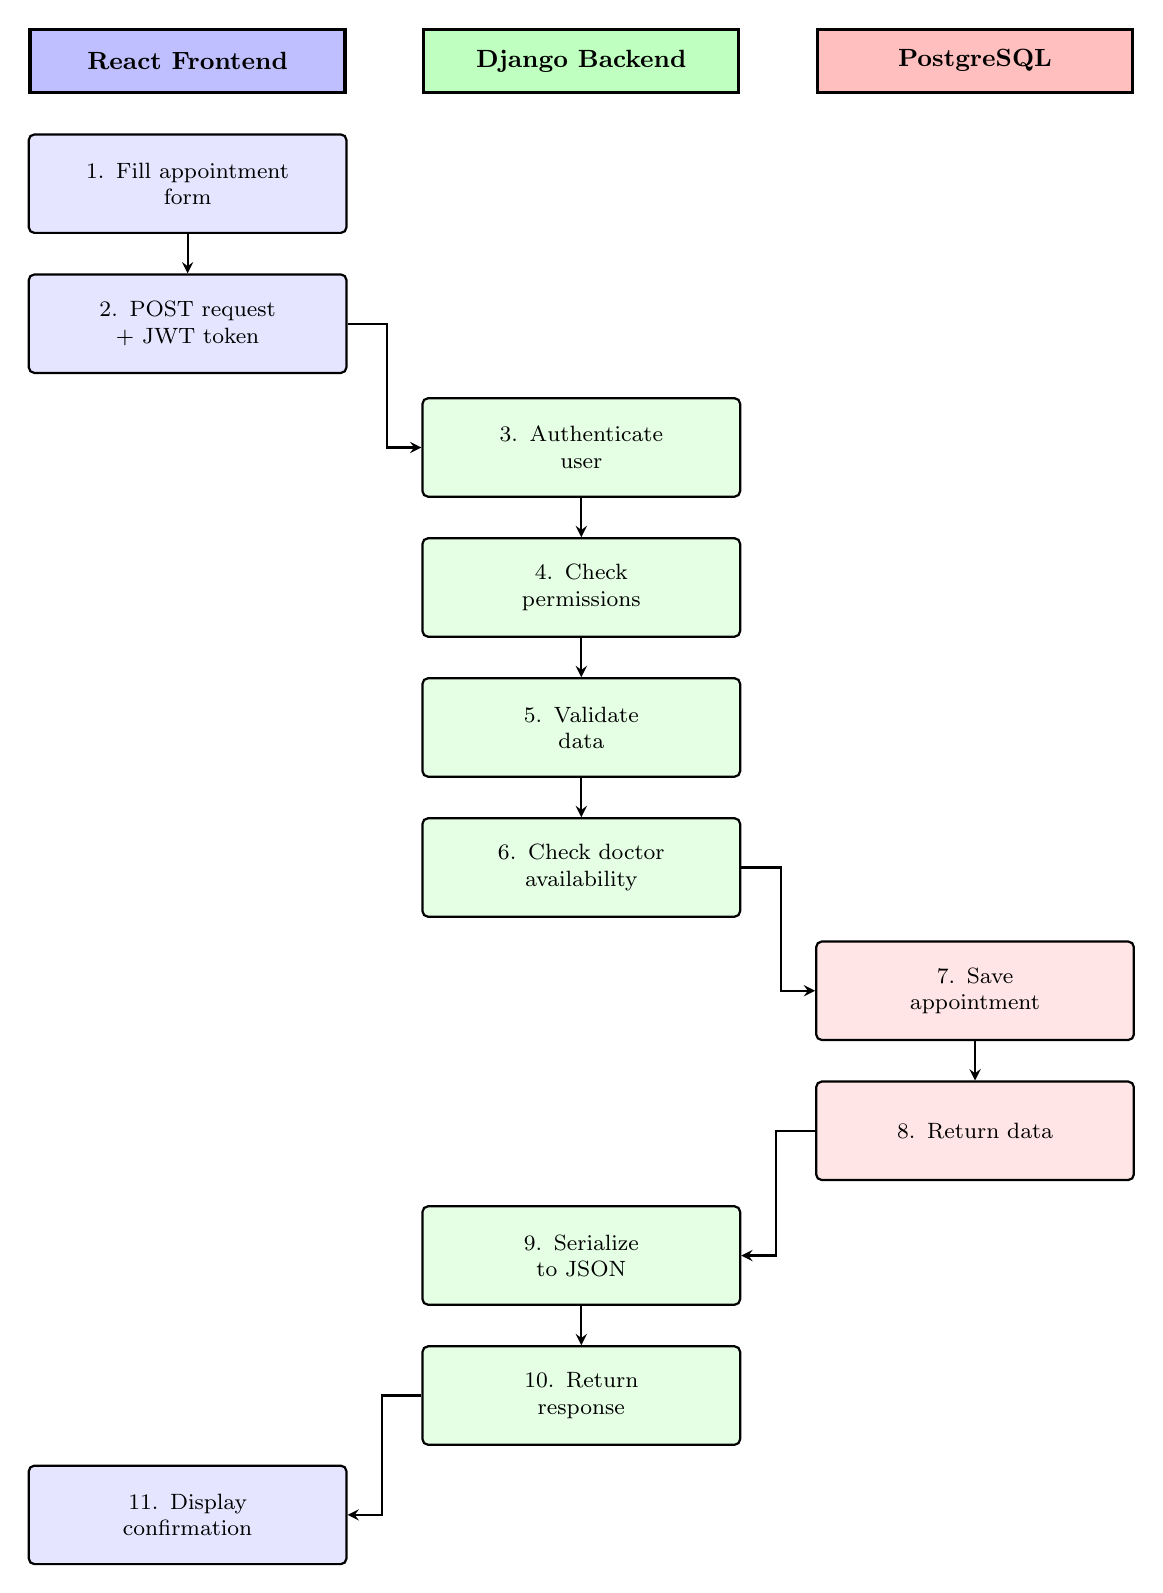
\begin{tikzpicture}[
    node distance=0.8cm,
    box/.style={
        rectangle,
        draw=black,
        thick,
        rounded corners=2pt,
        minimum width=4cm,
        minimum height=1.25cm,
        text width=3.8cm,
        align=center,
        font=\footnotesize
    },
    header/.style={
        rectangle,
        draw=black,
        very thick,
        minimum width=4cm,
        minimum height=0.8cm,
        font=\small\bfseries,
        align=center
    },
    arrow/.style={
        ->,
        thick,
        >=stealth
    }
]

% Column headers
\node[header, fill=blue!25] (h1) at (0, 0) {React Frontend};
\node[header, fill=green!25] (h2) at (5, 0) {Django Backend};
\node[header, fill=red!25] (h3) at (10, 0) {PostgreSQL};

% Frontend steps
\node[box, fill=blue!10, below=0.5cm of h1] (f1) {1. Fill appointment\\form};
\node[box, fill=blue!10, below=0.5cm of f1] (f2) {2. POST request\\+ JWT token};
\node[box, fill=blue!10, below=13.85cm of f2] (f11) {11. Display\\confirmation};

% Backend steps
\node[box, fill=green!10, below=3.85cm of h2] (b3) {3. Authenticate\\user};
\node[box, fill=green!10, below= 0.5cm of b3] (b4) {4. Check\\permissions};
\node[box, fill=green!10, below= 0.5cm of b4] (b5) {5. Validate\\data};
\node[box, fill=green!10, below= 0.5cm of b5] (b6) {6. Check doctor\\availability};
\node[box, fill=green!10, below=3.65cm of b6] (b9) {9. Serialize\\to JSON};
\node[box, fill=green!10, below =0.5cm of b9] (b10) {10. Return\\response};

% Database steps
\node[box, fill=red!10, below=10.75cm of h3] (d7) {7. Save\\appointment};
\node[box, fill=red!10, below= 0.5cm of d7] (d8) {8. Return data};

% Arrows
\draw[arrow] (f1) -- (f2);
\draw[arrow] (f2.east) -- ++(0.5,0) |- (b3.west);
\draw[arrow] (b3) -- (b4);
\draw[arrow] (b4) -- (b5);
\draw[arrow] (b5) -- (b6);
\draw[arrow] (b6.east) -- ++(0.5,0) |- (d7.west);
\draw[arrow] (d7) -- (d8);
\draw[arrow] (d8.west) -- ++(-0.5,0) |- (b9.east);
\draw[arrow] (b9) -- (b10);
\draw[arrow] (b10.west) -- ++(-0.5,0) |- (f11.east);

\end{tikzpicture}
\caption{Request Flow for Appointment Booking}
\label{fig:request-flow}
\end{figure}


This flow demonstrates how the three tiers work together: React handles user interaction, Django enforces business rules and validates permissions, and PostgreSQL ensures data persistence.
\clearpage

%------------ DB DESIGN ------------
\section{Database Design}

\subsection{Overview}
The database architecture for the healthcare web application follows a normalized relational model designed to support comprehensive medical data management while ensuring data integrity, security, and scalability. 

The design adheres to third normal form (3NF) to eliminate data redundancy and prevent update anomalies, which is critical in healthcare applications where data accuracy directly impacts patient care. All tables include timestamp fields (created\_at, updated\_at) for audit trails, and foreign key constraints with appropriate CASCADE and SET NULL behaviors ensure referential integrity throughout the system.

Our database design supports three primary user workflows: (1) patient self-service operations including appointment booking and medical history access, (2) doctor clinical workflows encompassing patient record management and prescription writing, and (3) administrative functions for user management and system monitoring. The schema maintains clear separation between authentication data (users table) and role-specific profile information (patients and doctors tables) to support future extensibility.


\subsection{Entity-Relationship Diagram}
Figure~\ref{fig:er-diagram} illustrates the database structure for the healthcare system. The design centers around a User entity that serves as the authentication base, with Patient and Doctor entities inheriting from it through an ISA relationship to store role-specific profile data. The schema supports core workflows: patients booking appointments with doctors, doctors creating medical records and prescriptions after appointments, and patients tracking their current medications with reminders. Additional entities handle medical document uploads. This nine-entity design implements all functional requirements from the requirements document while maintaining third normal form to ensure data integrity and minimize redundancy.

% [KEEP YOUR EXISTING ER DIAGRAM FIGURE HERE - DON'T CHANGE IT]

\begin{figure}[htbp] % [p] puts it on a separate page
\centering
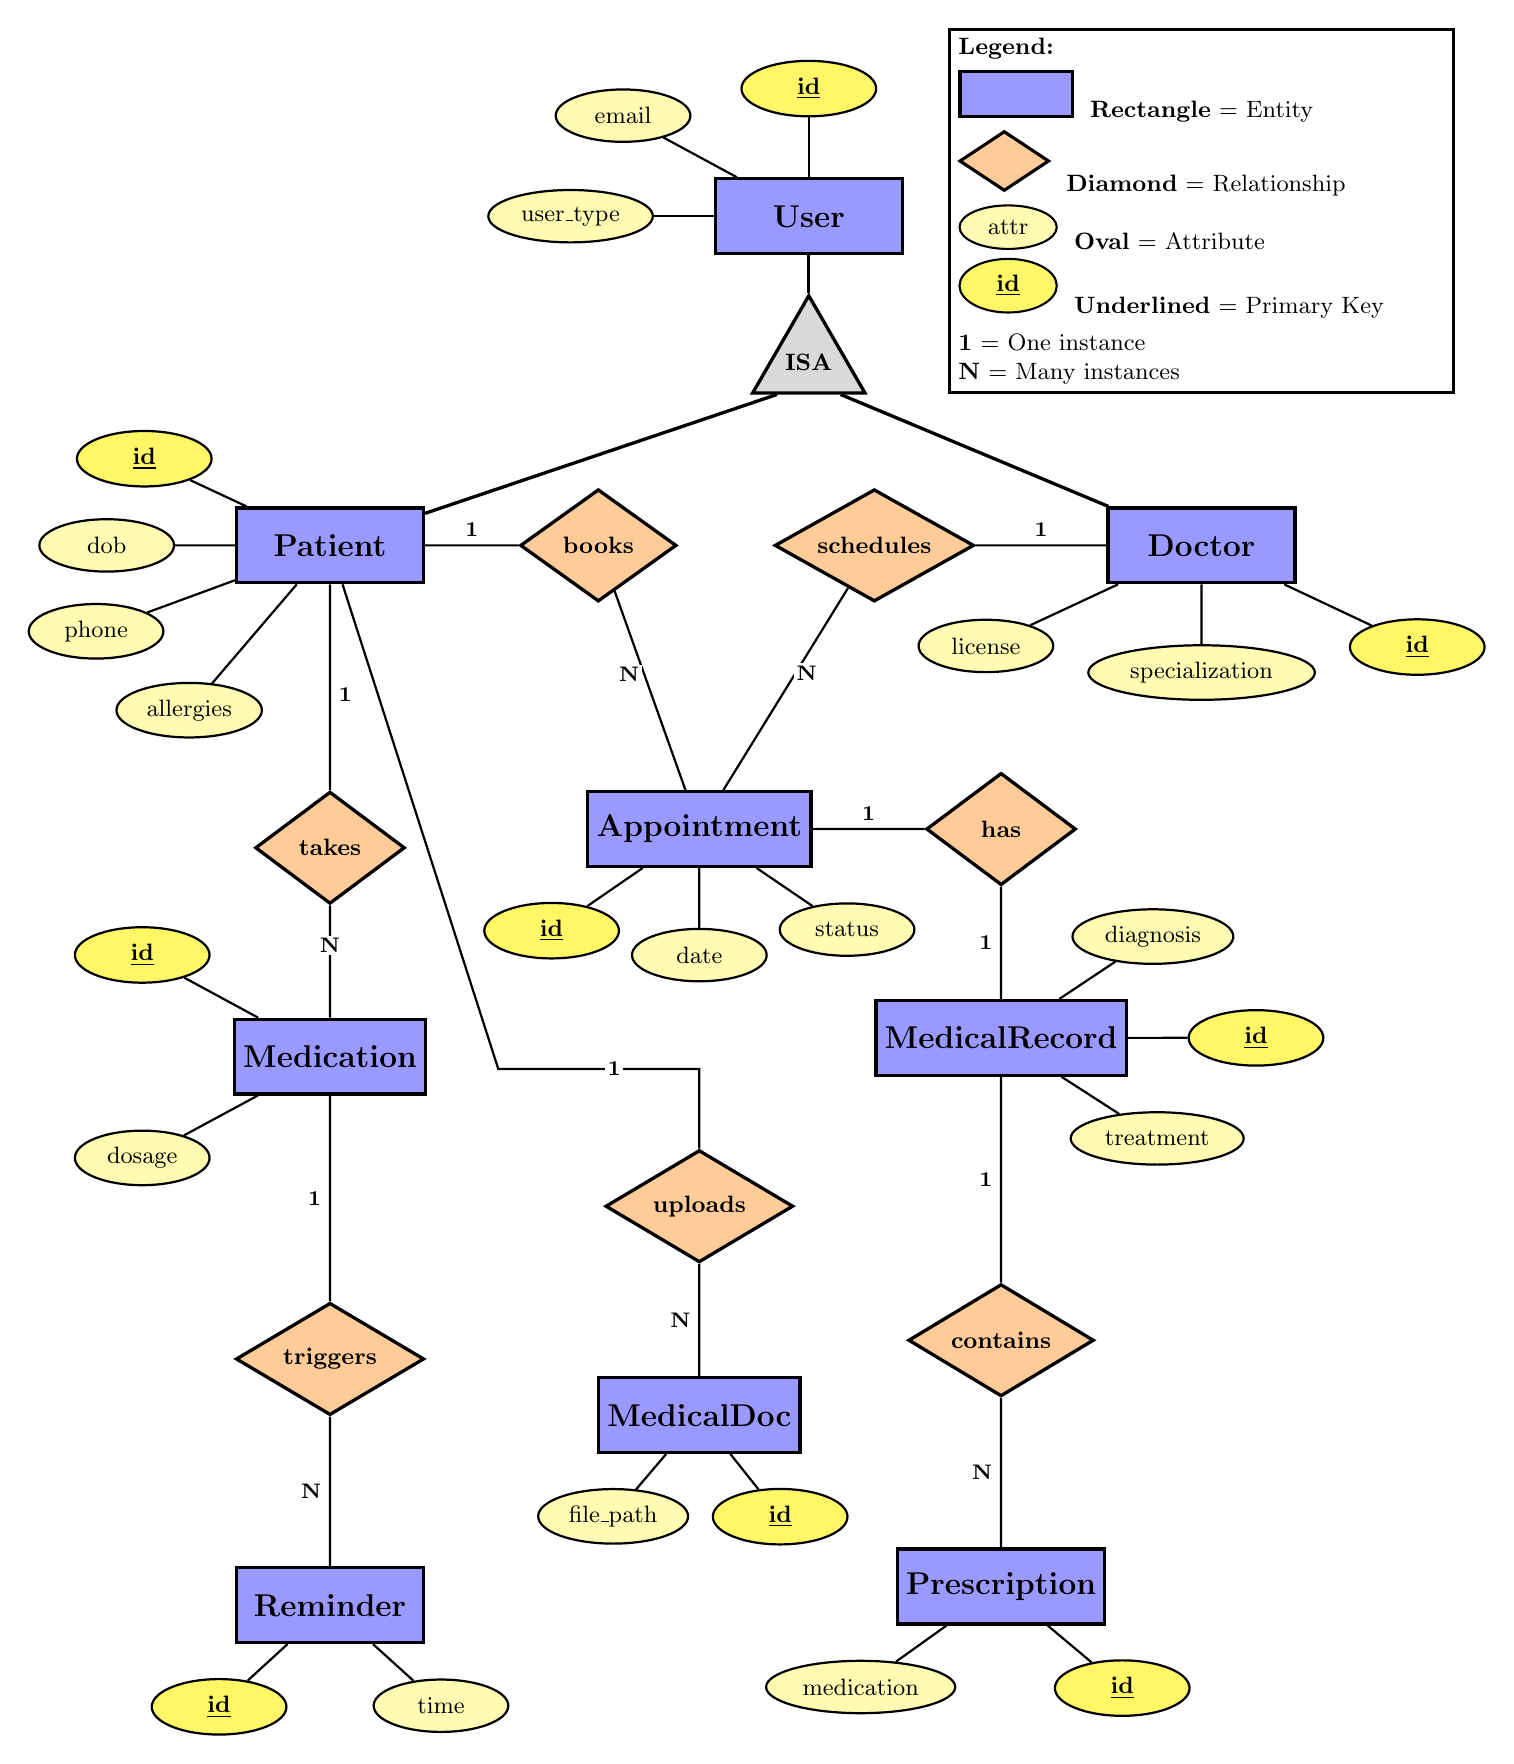
\begin{tikzpicture}[node distance=2.5cm and 3cm, scale=0.95, transform shape]

\tikzset{
    entity/.style={
        rectangle,
        draw=black,
        very thick,
        fill=blue!40,
        minimum width=2.5cm,
        minimum height=1cm,
        font=\bfseries\large
    },
    attribute/.style={
        ellipse,
        draw=black,
        thick,
        fill=yellow!30,
        minimum width=1.8cm,
        minimum height=0.7cm,
        font=\small
    },
    relationship/.style={
        diamond,
        draw=black,
        very thick,
        fill=orange!40,
        minimum width=2cm,
        minimum height=1.5cm,
        font=\bfseries\small,
        aspect=2
    },
    keyattr/.style={
        ellipse,
        draw=black,
        thick,
        fill=yellow!60,
        minimum width=1.8cm,
        minimum height=0.7cm,
        font=\small\bfseries
    },
    isa/.style={
        isosceles triangle,
        draw=black,
        very thick,
        fill=gray!30,
        minimum width=1.5cm,
        minimum height=1cm,
        isosceles triangle apex angle=60,
        shape border rotate=90
    },
    line/.style={
        draw,
        thick,
        -
    },
    cardinality/.style={
        font=\footnotesize\bfseries,
        fill=white,
        inner sep=1pt
    }
}

% ============== TOP SECTION: User ==============

\node[entity] (user) {User};
\node[keyattr, above=0.8cm of user] (user_id) {\underline{id}};
\node[attribute, above left=0.8cm of user] (user_email) {email};
\node[attribute, left=0.8cm of user] (user_type) {user\_type};

\draw[line] (user_id) -- (user);
\draw[line] (user_email) -- (user);
\draw[line] (user_type) -- (user);

% ============== ISA TRIANGLE ==============
\node[isa, below=.5cm of user] (isa_triangle) {};
\node[font=\small\bfseries] at (isa_triangle) {ISA};
\draw[line, very thick] (user) -- (isa_triangle);

% ============== PATIENT BRANCH (LEFT) ==============

\node[entity, below left=4.75cm of user,xshift=-0.5cm] (patient) {Patient};

\node[keyattr, above left=0.8cm of patient,yshift=-0.2cm] (patient_id) {\underline{id}};
\node[attribute, left=0.8cm of patient] (dob) {dob};
\node[attribute, below left=0.65cm of patient,xshift=-0.75cm,yshift=0.1cm] (phone) {phone};
\node[attribute, below left =2cm of patient,xshift=1.5cm] (allergies) {allergies};

\draw[line] (patient_id) -- (patient);
\draw[line] (dob) -- (patient);
\draw[line] (phone) -- (patient);
\draw[line] (allergies) -- (patient);
\draw[line, very thick] (isa_triangle.south west) -- (patient);

% ============== DOCTOR BRANCH (RIGHT) ==============

\node[entity, below right=4.75cm of user,xshift=-0.65cm] (doctor) {Doctor};

\node[keyattr, below right=0.8cm of doctor,xshift=0.4cm] (doctor_id) {\underline{id}};
\node[attribute, below left=0.8cm of doctor,xshift=-0.4cm] (license) {license};
\node[attribute, below=0.8cm of doctor] (specialization) {specialization};

\draw[line] (doctor_id) -- (doctor);
\draw[line] (license) -- (doctor);
\draw[line] (specialization) -- (doctor);
\draw[line, very thick] (isa_triangle.south east) -- (doctor);

% ============== APPOINTMENT (CENTER) ==============

\node[relationship, right=1.25cm of patient] (books) {books};
\node[relationship,  left=1.75cm of doctor] (schedules) {schedules};
\node[entity, below=2.5cm of books,xshift=1.35cm] (appointment) {Appointment};

\node[keyattr, below left=0.8cm of appointment,xshift=0.75cm] (appt_id) {\underline{id}};
\node[attribute, below=0.8cm of appointment] (appt_date) {date};
\node[attribute, below right=0.8cm of appointment, ,xshift=-0.75cm] (status) {status};

\draw[line] (patient) -- node[cardinality, above, yshift=2pt] {1} (books);
\draw[line] (books) -- node[cardinality, above, xshift=-8pt, yshift=2pt] {N} (appointment);
\draw[line] (doctor) -- node[cardinality, above, yshift=2pt] {1} (schedules);
\draw[line] (schedules) -- node[cardinality, above, xshift=8pt, yshift=2pt] {N} (appointment);
\draw[line] (appt_id) -- (appointment);
\draw[line] (appt_date) -- (appointment);
\draw[line] (status) -- (appointment);

% ============== MEDICAL RECORD ==============

\node[relationship, right=1.5cm of appointment] (has_record) {has};
\node[entity, below=1.5cm of has_record] (medrecord) {MedicalRecord};

\node[keyattr, right=0.8cm of medrecord] (record_id) {\underline{id}};
\node[attribute, above right=0.8cm of medrecord, xshift=-1cm] (diagnosis) {diagnosis};
\node[attribute, below right=0.8cm of medrecord, xshift=-1cm] (treatment) {treatment};

\draw[line] (appointment) -- node[cardinality, above, yshift=2pt] {1} (has_record);
\draw[line] (has_record) -- node[cardinality, left, xshift=-2pt] {1} (medrecord);
\draw[line] (record_id) -- (medrecord);
\draw[line] (diagnosis) -- (medrecord);
\draw[line] (treatment) -- (medrecord);

% ============== PRESCRIPTION (RIGHT OF RECORD) ==============

\node[relationship, below=2.75cm of medrecord] (contains) {contains};
\node[entity, below=2cm of contains] (prescription) {Prescription};

\node[keyattr, below right=0.8cm of prescription, xshift=-1cm] (presc_id) {\underline{id}};
\node[attribute, below left=0.8cm of prescription, xshift=1cm] (medication) {medication};

\draw[line] (medrecord) -- node[cardinality, left, xshift=-2pt] {1} (contains);
\draw[line] (contains) -- node[cardinality, left, xshift=-2pt] {N} (prescription);
\draw[line] (presc_id) -- (prescription);
\draw[line] (medication) -- (prescription);

% ============== MEDICATION (LEFT OF RECORD) ==============

\node[relationship, below=2.75cm of patient] (takes) {takes};
\node[entity, below=1.5cm of takes] (med) {Medication};

\node[keyattr, above left=0.8cm of med] (med_id) {\underline{id}};
\node[attribute, below left=0.8cm of med] (dosage) {dosage};

\draw[line] (patient) -- ++(0,-2) -| node[cardinality, near start, right, xshift=2pt] {1} (takes);
\draw[line] (takes) -- node[cardinality, above, yshift=2pt] {N} (med);
\draw[line] (med_id) -- (med);
\draw[line] (dosage) -- (med);

% ============== MEDICATION REMINDER ==============

\node[relationship, below=2.75cm of med] (triggers) {triggers};
\node[entity, below=2cm of triggers] (reminder) {Reminder};

\node[keyattr, below left=0.8cm of reminder,xshift=1cm] (rem_id) {\underline{id}};
\node[attribute, below right=0.8cm of reminder,xshift=-1cm] (rem_time) {time};

\draw[line] (med) -- node[cardinality, left, xshift=-2pt] {1} (triggers);
\draw[line] (triggers) -- node[cardinality, left, xshift=-2pt] {N} (reminder);
\draw[line] (rem_id) -- (reminder);
\draw[line] (rem_time) -- (reminder);

% ============== MEDICAL DOCUMENT ==============

\node[relationship, below=3.75cm of appointment] (uploads) {uploads};
\node[entity, below=1.5cm of uploads] (document) {MedicalDoc};

\node[keyattr, below right=0.8cm of document,xshift=-1.5cm] (doc_id) {\underline{id}};
\node[attribute, below left=0.8cm of document,xshift=1.5cm] (file_path) {file\_path};

\draw[line] (patient) -- ++(2.25,-7) -| node[cardinality, near start, right, xshift=2pt] {1} (uploads);
\draw[line] (uploads) -- node[cardinality, left, xshift=-2pt] {N} (document);
\draw[line] (doc_id) -- (document);
\draw[line] (file_path) -- (document);

% ============== LEGEND ==============

\node[draw=black, very thick, fill=white, text width=6.5cm, 
      above=1.5cm of doctor, font=\small] (legend) {
    \textbf{Legend:}\\[3pt]
    \tikz\node[entity, minimum width=1.5cm, minimum height=0.6cm] {};
    \textbf{ Rectangle} = Entity\\[2pt]
    \tikz\node[relationship, minimum width=1.2cm, minimum height=0.8cm] {};
    \textbf{ Diamond} = Relationship\\[2pt]
    \tikz\node[attribute, minimum width=1.3cm, minimum height=0.5cm] {attr};
    \textbf{ Oval} = Attribute\\[2pt]
    \tikz\node[keyattr, minimum width=1.3cm, minimum height=0.5cm] {\underline{id}};
    \textbf{ Underlined} = Primary Key\\[3pt]
    \textbf{1} = One instance\\
    \textbf{N} = Many instances
};

\end{tikzpicture}
\caption{Entity-Relationship Diagram for Healthcare Management System}
\label{fig:er-diagram}
\end{figure}

\subsection{Entity Relationships}

Table~\ref{tab:relationships} summarizes the relationships between entities and their cardinalities.

\begin{table}[h]
\centering
\begin{tabular}{|l|l|l|l|}
\hline
\textbf{From Entity} & \textbf{Relationship} & \textbf{To Entity} & \textbf{Cardinality} \\
\hline
User & ISA & Patient & 1:1 (inheritance) \\
User & ISA & Doctor & 1:1 (inheritance) \\
Patient & books & Appointment & 1:N \\
Doctor & schedules & Appointment & 1:N \\
Appointment & has & MedicalRecord & 1:1 \\
MedicalRecord & contains & Prescription & 1:N \\
Patient & takes & Medication & 1:N \\
Medication & triggers & Reminder & 1:N \\
Patient & uploads & MedicalDocument & 1:N \\
\hline
\end{tabular}
\caption{Entity Relationships and Cardinalities}
\label{tab:relationships}
\end{table}

% \subsection{Key Design Decisions}

% \begin{itemize}[leftmargin=*]
%     \item \textbf{ISA Inheritance:} 
%     User serves as the base authentication entity. \texttt{Patient} and \texttt{Doctor} extend \texttt{User} with role-specific data through one-to-one relationships, avoiding NULL values in a single table and maintaining a clean separation between authentication and profile data.
    
%     \item \textbf{Prescription vs Medication:} 
%     \texttt{Prescription} stores immutable historical records of doctor orders. \texttt{Medication} tracks current patient medication status, allowing patients to add non-prescribed medications (nullable \texttt{prescription\_id}). This separation supports audit trails and patient-managed medication tracking.
    
%     \item \textbf{PostgreSQL Features:} 
%     The design uses PostgreSQL's \texttt{array} type for \texttt{allergies} (native list storage) and \texttt{JSONB} type for \texttt{medical\_history} (flexible schema for varying patient data).
    
%     \item \textbf{Appointment Constraint:} 
%     \texttt{UNIQUE(doctor\_id, appointment\_date)} prevents double-booking of doctor time slots.
% \end{itemize}
\clearpage

\subsection{Relational Schema}

\subsubsection{User Authentication Schema}

\begin{lstlisting}[language=SQL, caption=User Table Schema]
CREATE TABLE users (
    id SERIAL PRIMARY KEY,
    email VARCHAR(255) UNIQUE NOT NULL,
    password VARCHAR(255) NOT NULL,
    first_name VARCHAR(100) NOT NULL,
    last_name VARCHAR(100) NOT NULL,
    user_type VARCHAR(20) NOT NULL 
        CHECK (user_type IN ('patient', 'doctor', 'admin')),
    is_active BOOLEAN DEFAULT true,
    created_at TIMESTAMP DEFAULT CURRENT_TIMESTAMP,
    updated_at TIMESTAMP DEFAULT CURRENT_TIMESTAMP
);

CREATE INDEX idx_users_email ON users(email);
\end{lstlisting}

\subsubsection{Patient and Doctor Schema}

\begin{lstlisting}[language=SQL, caption=Patient Table Schema]
CREATE TABLE patients (
    id SERIAL PRIMARY KEY,
    user_id INTEGER UNIQUE NOT NULL 
        REFERENCES users(id) ON DELETE CASCADE,
    date_of_birth DATE NOT NULL,
    phone_number VARCHAR(20),
    emergency_contact_name VARCHAR(100),
    emergency_contact_phone VARCHAR(20),
    allergies TEXT[] DEFAULT '{}',
    medical_history JSONB DEFAULT '{}',
    created_at TIMESTAMP DEFAULT CURRENT_TIMESTAMP,
    updated_at TIMESTAMP DEFAULT CURRENT_TIMESTAMP
);

CREATE INDEX idx_patients_user ON patients(user_id);
\end{lstlisting}

\begin{lstlisting}[language=SQL, caption=Doctor Table Schema]
CREATE TABLE doctors (
    id SERIAL PRIMARY KEY,
    user_id INTEGER UNIQUE NOT NULL 
        REFERENCES users(id) ON DELETE CASCADE,
    license_number VARCHAR(50) UNIQUE NOT NULL,
    specialization VARCHAR(100) NOT NULL,
    years_experience INTEGER DEFAULT 0,
    created_at TIMESTAMP DEFAULT CURRENT_TIMESTAMP,
    updated_at TIMESTAMP DEFAULT CURRENT_TIMESTAMP
);

CREATE INDEX idx_doctors_license ON doctors(license_number);
\end{lstlisting}

\subsubsection{Appointment and Medical Record Schema}

\begin{lstlisting}[language=SQL, caption=Appointment Table Schema]
CREATE TABLE appointments (
    id SERIAL PRIMARY KEY,
    patient_id INTEGER NOT NULL 
        REFERENCES patients(id) ON DELETE CASCADE,
    doctor_id INTEGER NOT NULL 
        REFERENCES doctors(id) ON DELETE CASCADE,
    appointment_date TIMESTAMP NOT NULL,
    status VARCHAR(20) DEFAULT 'scheduled' 
        CHECK (status IN ('scheduled', 'confirmed', 
                         'completed', 'cancelled')),
    reason TEXT,
    notes TEXT,
    created_at TIMESTAMP DEFAULT CURRENT_TIMESTAMP,
    updated_at TIMESTAMP DEFAULT CURRENT_TIMESTAMP,
    CONSTRAINT unique_doctor_time 
        UNIQUE(doctor_id, appointment_date)
);

CREATE INDEX idx_appointments_patient ON appointments(patient_id);
CREATE INDEX idx_appointments_doctor ON appointments(doctor_id);
CREATE INDEX idx_appointments_date ON appointments(appointment_date);
\end{lstlisting}

\begin{lstlisting}[language=SQL, caption=Medical Record Table Schema]
CREATE TABLE medical_records (
    id SERIAL PRIMARY KEY,
    appointment_id INTEGER UNIQUE NOT NULL 
        REFERENCES appointments(id) ON DELETE CASCADE,
    doctor_id INTEGER NOT NULL REFERENCES doctors(id),
    diagnosis TEXT NOT NULL,
    symptoms TEXT,
    treatment_notes TEXT,
    created_at TIMESTAMP DEFAULT CURRENT_TIMESTAMP,
    updated_at TIMESTAMP DEFAULT CURRENT_TIMESTAMP
);

CREATE INDEX idx_medical_records_appointment 
    ON medical_records(appointment_id);
\end{lstlisting}

\subsubsection{Prescription and Medication Schema}

\begin{lstlisting}[language=SQL, caption=Prescription Table Schema]
CREATE TABLE prescriptions (
    id SERIAL PRIMARY KEY,
    medical_record_id INTEGER NOT NULL 
        REFERENCES medical_records(id) ON DELETE CASCADE,
    medication_name VARCHAR(200) NOT NULL,
    dosage VARCHAR(100) NOT NULL,
    frequency VARCHAR(100) NOT NULL,
    duration VARCHAR(100),
    instructions TEXT,
    created_at TIMESTAMP DEFAULT CURRENT_TIMESTAMP
);

CREATE INDEX idx_prescriptions_record 
    ON prescriptions(medical_record_id);
\end{lstlisting}

\begin{lstlisting}[language=SQL, caption=Medication and Reminder Tables]
CREATE TABLE medications (
    id SERIAL PRIMARY KEY,
    patient_id INTEGER NOT NULL 
        REFERENCES patients(id) ON DELETE CASCADE,
    prescription_id INTEGER 
        REFERENCES prescriptions(id) ON DELETE SET NULL,
    name VARCHAR(200) NOT NULL,
    dosage VARCHAR(100) NOT NULL,
    frequency VARCHAR(100) NOT NULL,
    start_date DATE NOT NULL,
    end_date DATE,
    is_active BOOLEAN DEFAULT true
);

CREATE TABLE medication_reminders (
    id SERIAL PRIMARY KEY,
    medication_id INTEGER NOT NULL 
        REFERENCES medications(id) ON DELETE CASCADE,
    reminder_time TIME NOT NULL,
    is_enabled BOOLEAN DEFAULT true,
    last_reminded_at TIMESTAMP
);

CREATE INDEX idx_medications_patient ON medications(patient_id);
CREATE INDEX idx_reminders_medication 
    ON medication_reminders(medication_id);
\end{lstlisting}

\subsubsection{Medical Document Schema}

\begin{lstlisting}[language=SQL, caption=Medical Document Table Schema]
CREATE TABLE medical_documents (
    id SERIAL PRIMARY KEY,
    patient_id INTEGER NOT NULL 
        REFERENCES patients(id) ON DELETE CASCADE,
    uploaded_by_doctor_id INTEGER REFERENCES doctors(id),
    document_type VARCHAR(50) NOT NULL 
        CHECK (document_type IN ('X-ray', 'MRI', 
                                 'Lab Report', 'Other')),
    file_path VARCHAR(500) NOT NULL,
    description TEXT,
    upload_date TIMESTAMP DEFAULT CURRENT_TIMESTAMP
);

CREATE INDEX idx_medical_docs_patient 
    ON medical_documents(patient_id);
\end{lstlisting}

\clearpage

% -------------------API SECTION----------------------
\section{API Specification}

\subsection{Overview}

The healthcare application provides RESTful API endpoints for communication between the React frontend and Django backend. All endpoints use JSON for data exchange and require token-based authentication except for registration and login.


\subsection{Authentication Endpoints}

\begin{enumerate}
    \item \textbf{POST /api/auth/register/} : Register a new user account. No authentication required.
    \item \textbf{POST /api/auth/login/} : Authenticate user and receive access token. No authentication required.
    \item \textbf{POST /api/auth/logout/} : Invalidate current authentication token. Authentication required.
\end{enumerate}

\subsection{Patient Endpoints}

\begin{enumerate}
    \item \textbf{GET /api/patients/<id>/} : Retrieve patient profile. Patient can view own profile, doctors can view patient profiles.
    \item \textbf{PATCH /api/patients/<id>/} : Update patient profile information. Only the patient can update their own profile.
\end{enumerate}

\subsection{Doctor Endpoints}

\begin{enumerate}
    \item \textbf{GET /api/doctors/} : Get list of all doctors for appointment booking. Optional query parameter: \texttt{specialization}.
    \item \textbf{GET /api/doctors/<id>/} : Retrieve specific doctor profile information.
\end{enumerate}

\subsection{Appointment Endpoints}

\begin{enumerate}
    \item \textbf{GET /api/appointments/} : Get appointments for logged-in user. Patients see their appointments, doctors see appointments with them. Optional query parameters: \texttt{status}, \texttt{date}.
    \item \textbf{POST /api/appointments/} : Book a new appointment. Only patients can create appointments.
    \item \textbf{PATCH /api/appointments/<id>/} : Update appointment status or details. Patients can cancel/reschedule, doctors can update status.
\end{enumerate}

\subsection{Medical Record Endpoints}

\begin{enumerate}
    \item \textbf{GET /api/patients/<patient\_id>/medical-records/} : Get all medical records for a patient. Patient can view own records, doctors can view patient records.
    \item \textbf{POST /api/medical-records/} : Create medical record after appointment. Only doctors can create records.
\end{enumerate}

\subsection{Prescription Endpoints}

\begin{enumerate}
    \item \textbf{POST /api/prescriptions/} : Create prescription as part of medical record. Only doctors can create prescriptions.
    \item \textbf{GET /api/patients/<patient\_id>/prescriptions/} : Get all prescriptions for a patient.
\end{enumerate}

\subsection{Medication Endpoints}

\begin{enumerate}
    \item \textbf{GET /api/medications/} : Get current medications for logged-in patient. Optional query parameter: \texttt{is\_active} (default: true).
    \item \textbf{POST /api/medications/} : Add medication to patient's tracking list. Only patients can add.
\end{enumerate}

\subsection{Medical Document Endpoints}

\begin{enumerate}
    \item \textbf{POST /api/medical-documents/} : Upload medical document (X-ray, PDF, etc.). Patients and doctors can upload. Request uses multipart/form-data with fields: \texttt{patient}, \texttt{document\_type}, \texttt{file}, \texttt{description}.
    \item \textbf{GET /api/patients/<patient\_id>/documents/} : Get all medical documents for a patient with download URLs.
\end{enumerate}

\subsection{Admin Endpoints}

\begin{enumerate}
    \item \textbf{GET /api/admin/users/} : Get list of all system users. Admin only.
    \item \textbf{PATCH /api/admin/users/<id>/deactivate/} : Deactivate a user account. Admin only.
\end{enumerate}

\subsection{Response Codes}

\begin{itemize}
    \item \texttt{200 OK}: Successful request
    \item \texttt{201 Created}: Resource created
    \item \texttt{400 Bad Request}: Invalid data
    \item \texttt{401 Unauthorized}: Authentication required
    \item \texttt{403 Forbidden}: Insufficient permissions
    \item \texttt{404 Not Found}: Resource not found
    \item \texttt{409 Conflict}: Request conflicts with current state
\end{itemize}

% \subsection{API Summary}

% Table~\ref{tab:api-summary} provides a quick reference of all endpoints.

% \begin{table}[htbp]
% \centering
% \small
% \begin{tabular}{|l|l|l|}
% \hline
% \textbf{Endpoint} & \textbf{Method} & \textbf{Purpose} \\
% \hline
% /auth/register/ & POST & Register user \\
% /auth/login/ & POST & User login \\
% /auth/logout/ & POST & User logout \\
% \hline
% /patients/<id>/ & GET, PATCH & Patient profile \\
% /doctors/ & GET & List doctors \\
% /doctors/<id>/ & GET & Doctor profile \\
% \hline
% /appointments/ & GET, POST & Appointments \\
% /appointments/<id>/ & GET, PATCH & Appointment details \\
% \hline
% /patients/<id>/medical-records/ & GET & Medical records \\
% /medical-records/ & POST & Create record \\
% \hline
% /prescriptions/ & POST & Create prescription \\
% /patients/<id>/prescriptions/ & GET & List prescriptions \\
% \hline
% /medications/ & GET, POST & Medications \\
% /medical-documents/ & POST & Upload document \\
% /patients/<id>/documents/ & GET & List documents \\
% \hline
% /admin/users/ & GET & List users (admin) \\
% /admin/users/<id>/deactivate/ & PATCH & Deactivate user \\
% \hline
% \end{tabular}
% \caption{API Endpoints Summary}
% \label{tab:api-summary}
% \end{table}
\clearpage


% -------- UI/UX ---------
\section{UI/UX Mockups}
The user interface design focuses on creating intuitive and accessible interfaces for users. All mockups were created using Figma and emphasize clean layouts, clear navigation, and responsive design principles.

\begin{tcolorbox}[colback=gray!5,colframe=gray!40,boxrule=0.4pt,rounded corners]
\textbf{Figma Project:} \href{https://www.figma.com/design/KFYqF112j4akQXqaCOmpJ2/CUROVA-Healthcare-Website-homepage-UI?node-id=0-1&t=IstFX2OcNhijtQVr-1}{Healthcare Web Application UI}
\end{tcolorbox}


% \subsection{Registration Page}
% Facilitates new user registration with appropriate data collection and validation.

\begin{figure}[h]
    \centering
    
\includegraphics[width=0.7\textwidth]{D2/figma_mockups/Registration.png}
    \caption{Registration Page Design}
    \label{fig:registration}
\end{figure}

% \subsection{Login Page}
% Provides secure authentication interface for all user types.

\begin{figure}[h]
    \centering
    
\includegraphics[width=0.7\textwidth]{D2/figma_mockups/Login.png}
    \caption{Login Page Design}
    \label{fig:login}
\end{figure}


% \subsection{Homepage}
% The homepage serves as the primary entry point, providing system overview and navigation to key features.

\begin{figure}[h]
    \centering
    
\includegraphics[width=0.8\textwidth]{D2/figma_mockups/Home Page.png}
    \caption{Homepage Design}
    \label{fig:homepage}
\end{figure}

% \subsection{Appointment Page}
% Displays all appointments in an interactive calendar view for efficient schedule management.

\begin{figure}[h]
    \centering
    
\includegraphics[width=0.85\textwidth]{D2/figma_mockups/Appointment.png}
    \caption{Appointment Page Design}
    \label{fig:appointment-page}
\end{figure}

% \subsection{Patient Page}
% Lists all patients with search and filtering capabilities for quick access to patient information.

\begin{figure}[h]
    \centering
    
\includegraphics[width=0.85\textwidth]{D2/figma_mockups/Patient.png}
    \caption{Patient Page Design}
    \label{fig:patient-page}
\end{figure}

% \subsection{Admin Dashboard}
% Provides comprehensive system oversight and management tools for administrators.

\begin{figure}[h]
    \centering
    
\includegraphics[width=0.85\textwidth]{D2/figma_mockups/Dashboard.png}
    \caption{Admin Dashboard Design}
    \label{fig:admin-dashboard}
\end{figure}


\clearpage

\section{Security Architecture}

\subsection{Overview}

The healthcare application implements security measures to protect patient data through authentication, authorization, data encryption, and protection against common vulnerabilities. This design addresses the security requirements specified in our requirements document.

\subsection{Authentication}

The system uses token-based authentication provided by Django REST Framework.

\noindent
\textbf{How it works:}
\begin{enumerate}
    \item User logs in with email and password
    \item Backend verifies credentials and generates a token
    \item Token is returned to frontend and stored in browser
    \item Frontend includes token in all subsequent requests
    \item Backend validates token before processing each request
\end{enumerate}
\noindent
\textbf{Security measures:}
\begin{itemize}
    \item Passwords hashed using Django's PBKDF2 algorithm (not stored in plain text)
    \item All communication over HTTPS to prevent interception
    \item Tokens can be invalidated on logout
\end{itemize}

\subsection{Authorization}

Authorization controls what authenticated users can access based on their role (patient, doctor, admin).

\subsubsection{Role-Based Access Control}

The system implements three permission classes:
\begin{itemize}
    \item \textbf{IsPatient}: Only patients can access patient-specific endpoints
    \item \textbf{IsDoctor}: Only doctors can access doctor-specific endpoints
    \item \textbf{IsAdmin}: Only admins can access administrative functions
    \item \textbf{IsOwnerOrDoctor}: Patients access own data, doctors access patient data
\end{itemize}

\subsubsection{Access Control Matrix}

Table~\ref{tab:access-control} shows what each user role can do.

\begin{table}[htbp]
\centering
\small
\begin{tabular}{|l|c|c|c|}
\hline
\textbf{Resource} & \textbf{Patient} & \textbf{Doctor} & \textbf{Admin} \\
\hline
Own Profile & Read, Update & - & - \\
Other Profiles & - & Read & Read \\
Appointments & Create, Read, Cancel & Read, Update & - \\
Medical Records & Read (own) & Create, Read & - \\
Prescriptions & Read (own) & Create & - \\
Documents & Upload, Read (own) & Upload, Read & - \\
User Management & - & - & Full Access \\
\hline
\end{tabular}
\caption{User Role Permissions}
\label{tab:access-control}
\end{table}
\noindent
\textbf{Example:} When a patient tries to access \texttt{/api/patients/10/}, the system checks if they own that patient record. If not, it returns \texttt{403 Forbidden}.

\subsection{Data Protection}

\subsubsection{Encryption}

\textbf{Data in Transit:}
\begin{itemize}
    \item HTTPS required for all communication between browser and server
    \item Prevents eavesdropping and tampering with data
\end{itemize}
\noindent
\textbf{Data at Rest:}
\begin{itemize}
    \item Passwords stored hashed, never in plain text
    \item Database credentials stored in environment variables (not in code)
    \item Sensitive files excluded from version control using .gitignore
\end{itemize}

\subsubsection{Input Validation}

User inputs are validated to ensure data quality and prevent malicious entries:
\begin{itemize}
    \item Django serializers validate data types and required fields
    \item Email format checked during registration
    \item Date/time format validated for appointments
    \item File uploads restricted to PDF, JPG, PNG only
    \item Maximum file size limit of 5MB
\end{itemize}

\subsection{Protection Against Common Vulnerabilities}

As required by the capstone guidelines, the system protects against at least two common vulnerabilities.

\subsubsection{SQL Injection Prevention}

\textbf{What it is:} Attackers try to inject malicious database commands through user inputs.

\noindent
\textbf{How we prevent it:} Django ORM automatically uses parameterized queries. User inputs are never directly inserted into SQL statements.

\noindent
\textbf{Example:}
\begin{verbatim}
# Safe: Django ORM parameterized query
Patient.objects.filter(phone_number=user_input)

# Unsafe: Never used in our system
"SELECT * FROM patients WHERE phone='" + user_input + "'"
\end{verbatim}

\subsubsection{Unauthorized Access Prevention}

\textbf{What it is:} Users trying to access data they shouldn't by changing URLs or request parameters.

\noindent
\textbf{How we prevent it:}
\begin{itemize}
    \item All endpoints except login/register require authentication
    \item Permission classes check user role before processing requests
    \item Object-level checks verify ownership (patients can't see other patients' data)
    \item Invalid access attempts return \texttt{403 Forbidden}
\end{itemize}

\noindent
\textbf{Example:} Patient changes URL from \texttt{/api/patients/5/} to \texttt{/api/patients/10/}. Backend verifies ownership and blocks access if the patient doesn't own record 10.

\subsection{Additional Security Measures}

\textbf{Cross-Site Request Forgery (CSRF) Protection:}
\begin{itemize}
    \item Django CSRF middleware enabled
    \item CSRF tokens required for state-changing operations
    \item CORS configured to allow requests only from trusted frontend
\end{itemize}
\noindent
\textbf{Cross-Site Scripting (XSS) Protection:}
\begin{itemize}
    \item Django automatically escapes output
    \item React escapes variables by default
    \item User-generated content sanitized
\end{itemize}

\subsection{Summary}

The security architecture protects patient data through multiple layers: token-based authentication verifies user identity, role-based authorization controls access to resources, HTTPS encryption protects data during transmission, and input validation prevents malicious data entry. The system implements protections against SQL injection and unauthorized access as required by the capstone guidelines.

\clearpage

% % ------ Updatet Timeline ------
% \section{Updated Project Timeline}

% Table~\ref{tab:timeline} presents the updated project timeline.

% \begin{table}[htbp]
% \centering
% \begin{tabular}{|l|l|l|}
% \hline
% \textbf{Week} & \textbf{Deliverable} & \textbf{Deadline} \\
% \hline
% Week 2 & D1: Requirements & September 17, 2025 \\
% Week 4 & D2: Design & October 12, 2025 \\
% Week 6 & D3: Backend MVP & October 26, 2025 \\
% Week 8 & D4: Frontend Integration & November 9, 2025 \\
% Week 10-12 & D5: Deployment & November 23-30, 2025 \\
% \hline
% \end{tabular}
% \caption{Updated Project Timeline}
% \label{tab:timeline}
% \end{table}


\end{document}